\documentclass[tikz,border=8pt]{standalone}
\usepackage{tikz}
\usetikzlibrary{shapes,arrows,positioning}
\tikzstyle{proc}=[rectangle,draw,rounded corners,fill=blue!10,align=center,minimum width=3.4cm,minimum height=0.9cm,font=\small]
\tikzstyle{dec}=[diamond,draw,fill=green!10,align=center,aspect=2,font=\small]
\tikzstyle{term}=[rectangle,draw,rounded corners=8pt,fill=gray!15,align=center,minimum width=2.6cm,minimum height=0.9cm,font=\small\bfseries]
\tikzstyle{arr}=[->,thick]
\begin{document}
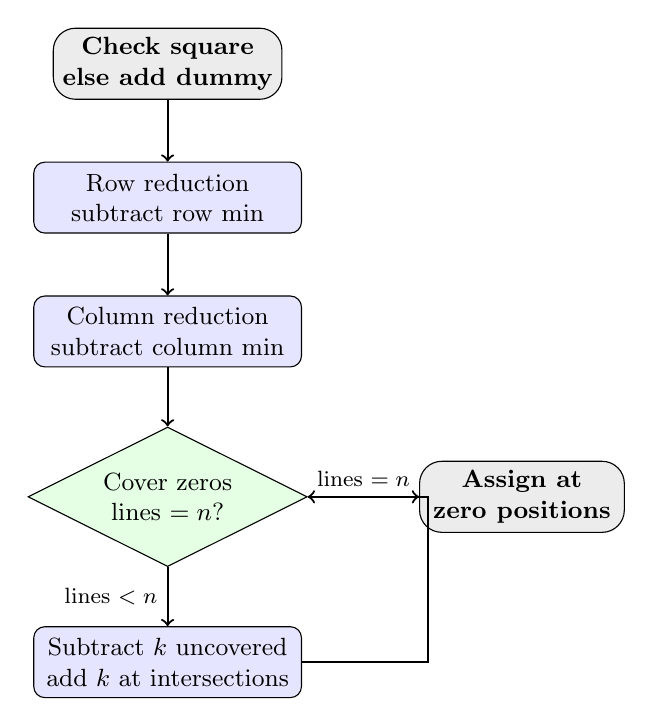
\begin{tikzpicture}[node distance=1.7cm]
\node[term] (A) {Check square\\else add dummy};
\node[proc, below of=A] (B) {Row reduction\\subtract row min};
\node[proc, below of=B] (C) {Column reduction\\subtract column min};
\node[dec, below of=C, yshift=-0.4cm] (D) {Cover zeros\\lines $=n$?};
\node[term, right of=D, xshift=2.8cm] (E) {Assign at\\zero positions};
\node[proc, below of=D, yshift=-0.4cm] (F) {Subtract $k$ uncovered\\add $k$ at intersections};
\draw[arr] (A) -- (B);
\draw[arr] (B) -- (C);
\draw[arr] (C) -- (D);
\draw[arr] (D) -- node[above,font=\footnotesize]{lines $=n$} (E);
\draw[arr] (D) -- node[left,font=\footnotesize]{lines $<n$} (F);
\draw[arr] (F.east) -- ++(1.6,0) |- (D.east);
\end{tikzpicture}
\end{document}
